\documentclass{article}

\usepackage[T1]{fontenc}    %Schriftart des Dokumentes
\usepackage[ngerman]{babel} %Dokumentensprache, hier Deutsch
\usepackage{amsmath, amssymb, stmaryrd} %mathematische Schriftzeichen
\usepackage{graphicx} %Einfügen von Grafiken
\usepackage{wrapfig}
\usepackage{bm}

\setlength{\parindent}{0pt} %Einrückung von Absätzen auf null gesetzt
\setlength{\parskip}{10pt} %Abstand zischen Absätzen auf 10pt gesetzt

\title{Versuch 31: Optische Abbildungen}
\author{Matthias Kuntz}
\date{05.09.2023}

\begin{document}

\maketitle

%-------------------------EINLEITUNG-------------------------
\section{Einleitung}

Dieser Versuch dient einer Einführung in das Thema der Optische Abbildungen. In insgesamt vier Versuchsteilen werden die Eigenschaften von Linsen genauer betrachtet. Im ersten Teil nutzt man die Messung der Abstände zwischen Objekt, Linse und Bild in Positionen, die ein scharfes Bild ergeben, um grafisch die Brennweite der Linse zu bestimmen. Im zweiten Teil wird mithilfe des sogenannten Besselverfahrens über den Abstand der Positionen der Linse, bei denen ein scharfes Bild entsteht die Brennweite erfasst. Anschließend sollen im dritten Teil die beiden größten Fehlerquellen von Linsen untersucht werden, die chromatische Aberration und die sphärische Aberration, letztere aber nur qualitativ. Zum Schluss wird ein Aufbau eines Mikroskops verwendet um dessen Auflösungsvermögen zu bestimmen. 

\subsection{Physikalische Grundlagen}

Da Optische Abbildungen das Hauptthema dieses Versuches sind, sollen zunächst diese genauer erläutert werden. Als optische Abbildungen bezeichnet man Vorgänge, bei denen von einem Objektpunkt ausgehende Lichtbündel nach Durchgang durch ein optisches System, zum Beispiel einer Reihe von Linsen, wieder in einem Punkt, dem Bildpunkt, vereinigt werden. Eine wichtige Klassifizierung ist hierbei die der reellen und virtuellen Abbildungen. Reelle Abbildungen zeichnen sich darüber aus, dass sie im Allgemeinen im Schnittpunkt von Lichtbündeln entstehen, die vom gleichen Objektpunkt ausgehen, und somit auf einem Schirm abbildbar sind, während letztere im Schnittpunkt der rückwärtigen Verlängerung divergenter Lichtbündel enstehen, wie beispielsweise bei einem Spiegel, und somit nicht mit einem Schirm auffangbar sind.

Häufig werden für optische Abbildungen Linsen verwendet. Als Linsen bezeichnet man transparente Materialien, die dazu genutzt werden Licht zu brechen und Abbildungen zu erzeugen. Verschiedene Krümmungen der Linsenoberflächen sorgen hierbei für verschiedene Effekte. 

Für optische Abbildungen mit Linsen gilt die Abbildungsgleichung

\begin{equation}
    \frac{1}{f} = \frac{1}{g} + \frac{1}{b}
\end{equation}

die den Zusammenhang zwischen der Brennweite der Linse $f$ sowie den Größen Gegenstandsweite $g$, dem Abstand zwischen dem abgebildeten Gegenstand und der Linse, und Bildweite $b$, dem Abstand zwischen Linse und Abbildung, angibt.

Weitere wichtige Größen sind die Gegenstandsgröße $G$, ergo die Größe des abgebildeten Gegenstands, und die Bildgröße $B$, das Gegenstück zu $G$ und die Größe der Abbildung. Sie stehen direkt mit der Gegenstandsweite und der Bildweite im Zusammenhang, da der Quotiont aus beiden den Abbildungsmaßstab $\beta$ definiert:

\begin{equation}
    \beta = \frac{B}{G} = \frac{b}{g}
\end{equation}

Um die Brennweite $f$ einer Linse zu bestimmen gibt es mehrere Wege, einer davon ist die sogenannte Bessel-Methode. Für uns wird sie aufgrund ihrer Genauigkeit im Vergleich zur trivialen Messung bevorzugt. Hier wird ausgenutzt, dass es bei einem konstanten Abstand $L > 4f$ zwischen Bild und Gegenstand exakt zwei Linsenstellungen zwischen diesen gibt, bei denen die Abbildung scharf wird. Bestimmt man die Distanz $d$ zwischen diesen zwei Positionen, so ist die Brennweite gegeben durch:

\begin{equation}
    f = \frac{L^2 - d^2}{4L}
\end{equation}

Es lohnt sich noch kurz einen Blick auf die zwei größten Fehlerquellen von Linsen zu werfen. Diese sind die sphärische und die chromatische Aberration. Die Erstere entsteht aufgrund des Phänomens, dass achsenferne Lichtstrahlen an einer Linse anders gebrochen werden als achsennahe Strahlen und diese somit einen anderen Brennpunkt haben. Eine Minimierung dieses Fehlers kann durch das Verwenden einer Lochblende erziehlt werden, was aber die Lichtstärke beschränkt, oder durch eine spezielle asphärische Linse, welche in der Regel aber teurer sind. \\ Die chromatische Aberration entsteht, da generell der Brechungsindex $n$ abhängig von der Wellenlänge des Lichts ist. Da nun unterschiedliche Lichtfarben unterschiedliche Wellenlängen haben, werden verschiedene Farben anders stark gebrochen und weißes Licht, das aus Strahlen verschiedenster Wellenlängen besteht, wird in die unterschiedlichen Farben aufgespaltet. Da nun die Brennweite über die Formel

\begin{equation}
    \frac{1}{f} = (n-1) \left( \frac{1}{r_1} + \frac{1}{r_2} \right)
\end{equation}

nicht nur von den Radien $r_1$ und $r_2$ der Grenzfläche der Linse, sondern auch vom Brechungsindex abhängt, haben unterschiedliche Farben im Endeffekt unterschiedliche Brennpunkte. Zur Minimierung lässt sich erneut eine Lochblende, wieder mit dem Nachteil der reduzierten Lichtstärke, oder ein Achromat, ein Linsensystem mit unterschiedlicher Dispersion und Brechkraft, das die chromatischen Fehler destruktiv interferieren lässt, verwenden.

Möchte man einen kleinen Gegenstand möglicht stark vergrößern, wie bei einem Mikroskop, so muss der Sehwinkel vergrößert werden. Dies geschieht beispielsweise wenn man einen Gegenstand nah an sein Auge heranbringt, um ihn besser zu erkennen. Da die Linse im Auge aber nur bedingt variiert werden kann gibt es den Wert der Sehweite $s_0$. Dieser bestimmt die kleinste Distanz, auf die ein gesundes Auge einen Gegenstand über einen längeren Zeitraum ohne Anstrengung beobachten kann, er wurde festgelegt auf $s_0 = 25cm$. \\ Möchten kleinere Objekte detailreicher erkannt werden so benötigt man optische Instrumente, die den Sehwinkel und damit die Bildgröße vergrößern. Beispiele dafür sind Lupen und Mikroskope.

Ein Mikroskop besteht aus einem Objektiv und einem Okular, ergo zwei Linsen. Zunächst bildet das Objektiv den zu beobachtenden Gegenstand, der mit der Gegenstandsweite $g$ etwas über der Brennweite $f_1$ des Objektivs liegt, auf die Bildebene innerhalb des Mikroskops ab, wodurch ein sogenanntes Zwischenbild entsteht. Mit dem Okular wird dieses Zwischenbild dann wie mit einer Art Lupe betrachtet, das Zwischenbild liegt also genau im Brennpunkt des Okulars. Die gesamte Vergößerung $V_M$ eines Mikroskops ergibt sich dann mit:

\begin{equation}
    V_M = \frac{s_0 t}{f_1 f_2}
\end{equation}

Mit $t$ ist die sogenannte Tubuslänge gemeint, sie gibt den Abstand zwischen dem gegenstandsseitigen Objektivbrennpunkt und dem bildseitigen Okularbrennpunkt an. $s_0$ ist die Sehweite, $f_1$ die Brennweite vom Objektiv und $f_2$ die Brennweite vom Okular.

Allgemein ist die maximale Vergrößerung beschränkt durch die Wellennatur des Lichts. Verscuht man die Vergrößerung durch Anpassung der Brennweiten sowie der Tubuslänge zu extremieren, so treten Interferenzen in der Abbildung auf.

Hier ist die Auflösung wichtig. Sie gibt den minimalen Abstand an, bei dem zwei Punkte noch voneinander unterscheidbar sind. Das Rayleigh-Kriterium sagt aus, dass zwei Punkt nur dann voneinander unterscheidbar sind, wenn der Abstand der beiden Beugungsfiguren größer ist als die halbe Breite des zentralen Maximums. Somit liegt die Grenze dort, wo das Beugungsmaximum des einen Punkts in das Beugungsminimum des anderen Punkts fällt. Der minimale Abstand der Beugungsfiguren ist gegeben durch:

\begin{equation}
    B_{min} = 1,22 \frac{\lambda b}{D}
\end{equation}

Dabei ist $\lambda$ die Wellenlänge des Lichts, $b$ die Bildweite und $D$ der Durchmesser der Objektivlinse. Gleichung (6) kann dann noch umgeschrieben werden zum kleinsten Abstand zweier Objektpunkte:

\begin{equation}
    G_{min} = 1,22 \frac{\lambda g}{D} = 1,22 \frac{\lambda f}{D}
\end{equation}

Daraus folgt:

\begin{equation}
    G_{min} = 1,22 \frac{\lambda}{2n \sin{\alpha}} = 0,61 \frac{\lambda}{\text{NA}}
\end{equation}

Wobei $\alpha$ hier der halbe Öffnungswinkel der Objektivlinse ist, $n$ der Brechungsindex des Mediums zwischen Linse und Gegenstand und NA die numerische Apertur, die häufig auf Geräten angegeben ist.

Zur Bestimmung von $\alpha$ kann folgende Relation aus Abbildung 1 abgelesen werden und mit der Kleinwinkelnäherung genähert werden:

\begin{equation}
    \tan{\alpha} \approx \alpha = \frac{D/2}{f}
\end{equation}

\begin{figure} [h]
    \centering
    \includegraphics[width=6cm]{graphics/dia0.jpg}
    \caption{Zeichnung zur Bestimmung von $\alpha$}
\end{figure}

\newpage

\subsection{Versuchsaufbau}

Bei diesem Versuch werden vier verschiedene Versuchsaufbauten verwendet.

Beim ersten Versuchsteil werden eine Lampe, eine Dia mit Teststruktur, eine Achromatlinse und ein Schirm wie in Abbildung 2 zu sehen auf einer optischen Schiene mit Maßstab angebracht. Nun bestimmt man bei verschiedenen Gegenstandsweiten $g$ die Bildweite $b$ sodass das Bild auf dem Schirm scharf wird und misst dabei die Gegenstandsgröße $G$ und Bildgrößen $B$.

\begin{figure} [h!]
    \centering
    \includegraphics[width=6cm]{graphics/1.jpg}
    \caption{Skizze vom ersten Versuchsaufbau}
\end{figure}

Für den zweiten Teil werden Dia und der Schirm auf einen festen Abstand von $L \approx 5f$ eingestellt und mit einer bikonvexen Linse, dessen Brennweite $f$ genutzt wird um den Abstand $L$ zu bestimmen, werden die zwei Positionen zwischen Dia und Schirm gesucht, bei denen das Bild auf dem Schirm scharf wird, um den Abstand zwischen den beiden Positionen zu bestimmen. Diese Messung wird drei mal durchgeführt.

\begin{figure} [h!]
    \centering
    \includegraphics[width=6cm]{graphics/2.jpg}
    \caption{Skizze vom zweiten Versuchsaufbau}
\end{figure}

\newpage

Anschließend wird der Versuchsaufbau modifiziert, indem Lichtfilter vor der Lampe angebracht werden, sodass zuerst rotes und dann blaues Licht entsteht. Beide Male werden jeweils die Messungen von Aufbau zwei wiederholt. Anschließend wird qualitativ die sphärische Abberation mit einer Loch- und einer Ringblende untersucht, die vor der Linse angebracht werden.

\begin{figure} [h!]
    \centering
    \includegraphics[width=6cm]{graphics/3.jpg}
    \caption{Skizze vom dritten Versuchsaufbau}
\end{figure}

Zuletzt wird ein Aufbau eines Mikroskops wie in Abbildung 5 dargestellt verwendet. Dabei werden zunächst der Messpalt mit veränderlicher Spaltbreite, das Objektiv, der Schirm für das Zwischenbild und das Okular auf feste gegebene Abstände eingestellt. Vor der Lampe wird ein grüner Lichtfilter angebracht. Danach wird durch Schauen durch das Okular die Position der Dia mit Kreuzgitter so variiert, bis das Bild scharf ist. Zunächst bestimmt man mithilfe der gemessenen Größe des Zwischenbilds die Gittergröße des Kreuzgitters. Danach verkleinert man die Spaltgröße so weit, bis die senkrechten Strukturen des Gitters gerade so nicht mehr zu sehen sind. Diese Spaltbreite wird drei Mal gemessen. Zuletzt betrachtet man noch qualitativ die Auswirkungen auf die gemessene Spaltbreite bei rotem und blauem Licht.

\begin{figure} [h!]
    \centering
    \includegraphics[width=6cm]{graphics/4.jpg}
    \caption{Skizze vom vierten Versuchsaufbau}
\end{figure}

%---------------VERSUCHSPROTOKOLL MIT MESSDATEN---------------
\newpage

\section{Versuchsprotokoll mit Messdaten}

\includegraphics[width=\textwidth]{graphics/mess1.jpg}
\newpage
\includegraphics[width=\textwidth]{graphics/mess2.jpg}
\newpage
\includegraphics[width=\textwidth]{graphics/mess3.jpg}
\newpage

\addtocounter{table}{3}

%-------------------------AUSWERTUNG-------------------------
\section{Auswertung}

\subsection{Zu Aufgabe 1}

Zur Auswertung der Messdaten von Tabelle 1 wird Tabelle 4 angelegt.

\begin{table}[h]
\centering
\caption{Auswertung der Messdaten aus Tabelle 1}
\begin{tabular}{c|c|c|c|c|c}
\textbf{Nr.} & \textbf{$\bm{g}$} & \textbf{$\bm{b}$} & \textbf{Art} & \textbf{Richtung} & \textbf{$\bm{\beta}$} \\ \hline
    1 & $g > 2f$ & $g > b > f$ & reell & umgekehrt & $<1$ \\ \hline
    2 & $g = 2f$ & $2f = b > f$ & reell & umgekehrt & $\approx 1$ \\ \hline
    3 & $2f > g > f$ & $b > g > f$ & reell & umgekehrt & $>1$ \\ \hline
    4 & $g = f$ & $b > g = f$ & reell & umgekehrt & $\infty$ \\ \hline
    5 & $f > g$ & $f > g > b$ & reell & aufrecht & -
\end{tabular}
\end{table}

Der Abbildungsmaßstab wird jeweils mit Gleichung (2) bestimmt. Vergleicht man die Auswertung der Tabelle mit den in Abbildung 6 dargestellten optischen Abbildungen, so stimmen die Schlussfolgerungen überein.

Nun werden die gemessenen Werte für die Bild- und Gegenstandsweiten aus Tabelle 1 in ein Diagramm eingetragen (Abbildung 7), um die Brennweite grafisch zu bestimmen. Die Gegenstandsweiten werden auf der x-Achse aufgetragen und mit den zugehörigen Bildweiten auf der y-Achse verbunden. Der Schnittpunkt der Geraden wird mit der Brennweite identifiziert. 

Aus dem Diagramm liest man die Werte

\begin{equation}
    \begin{split}
        f_{graph_{1}} &= 10,0cm \\
        f_{graph_{2}} &= 10,1cm
    \end{split}
\end{equation}

ab und schätzt den Fehler von $f_{graph_{1}}$ und $f_{graph_{2}}$ wie im Diagramm eingezeichnet ab mit der Streuung der Schnittpunkte:

\begin{equation}
    \begin{split}
        \Delta f_{graph_{1}} &= 0,6cm \\
        \Delta f_{graph_{2}} &= 0,4cm
    \end{split}
\end{equation}

Berechnet man den Mittelwert der zwei abgelesenen Werte für $f_{graph_{1}}$ und $f_{graph_{2}}$ und berechnet den Fehler mit der Fehlerfortpflanzung so erhält man:

\begin{equation}
    \bm{f_{graph} = (10,1 \pm 0,4)cm}
\end{equation}

Vergleicht man diesen Wert mit den im Messprotokoll berechneten Wert von $f=(9,85 \pm 0,03)cm$ indem man die Differenz $D$ und den Fehler der Differenz $\Delta D$ berechnet, so stellt man fest, dass der Unterschied nicht signifikant ist:

\begin{equation}
    \begin{split}
        D &= 0,25cm \\
        \Delta D &= 0,40cm
    \end{split}
\end{equation}

$\implies \Delta D > D \implies \text{Unterschied nicht signifikant.}$

Es ergibt sich somit eine Abweichung von $\sigma = \frac{D}{\Delta D} = 0,63$, was noch innerhalb der $1\sigma$-Umgebung liegt.

\begin{figure} [p]
    \centering
    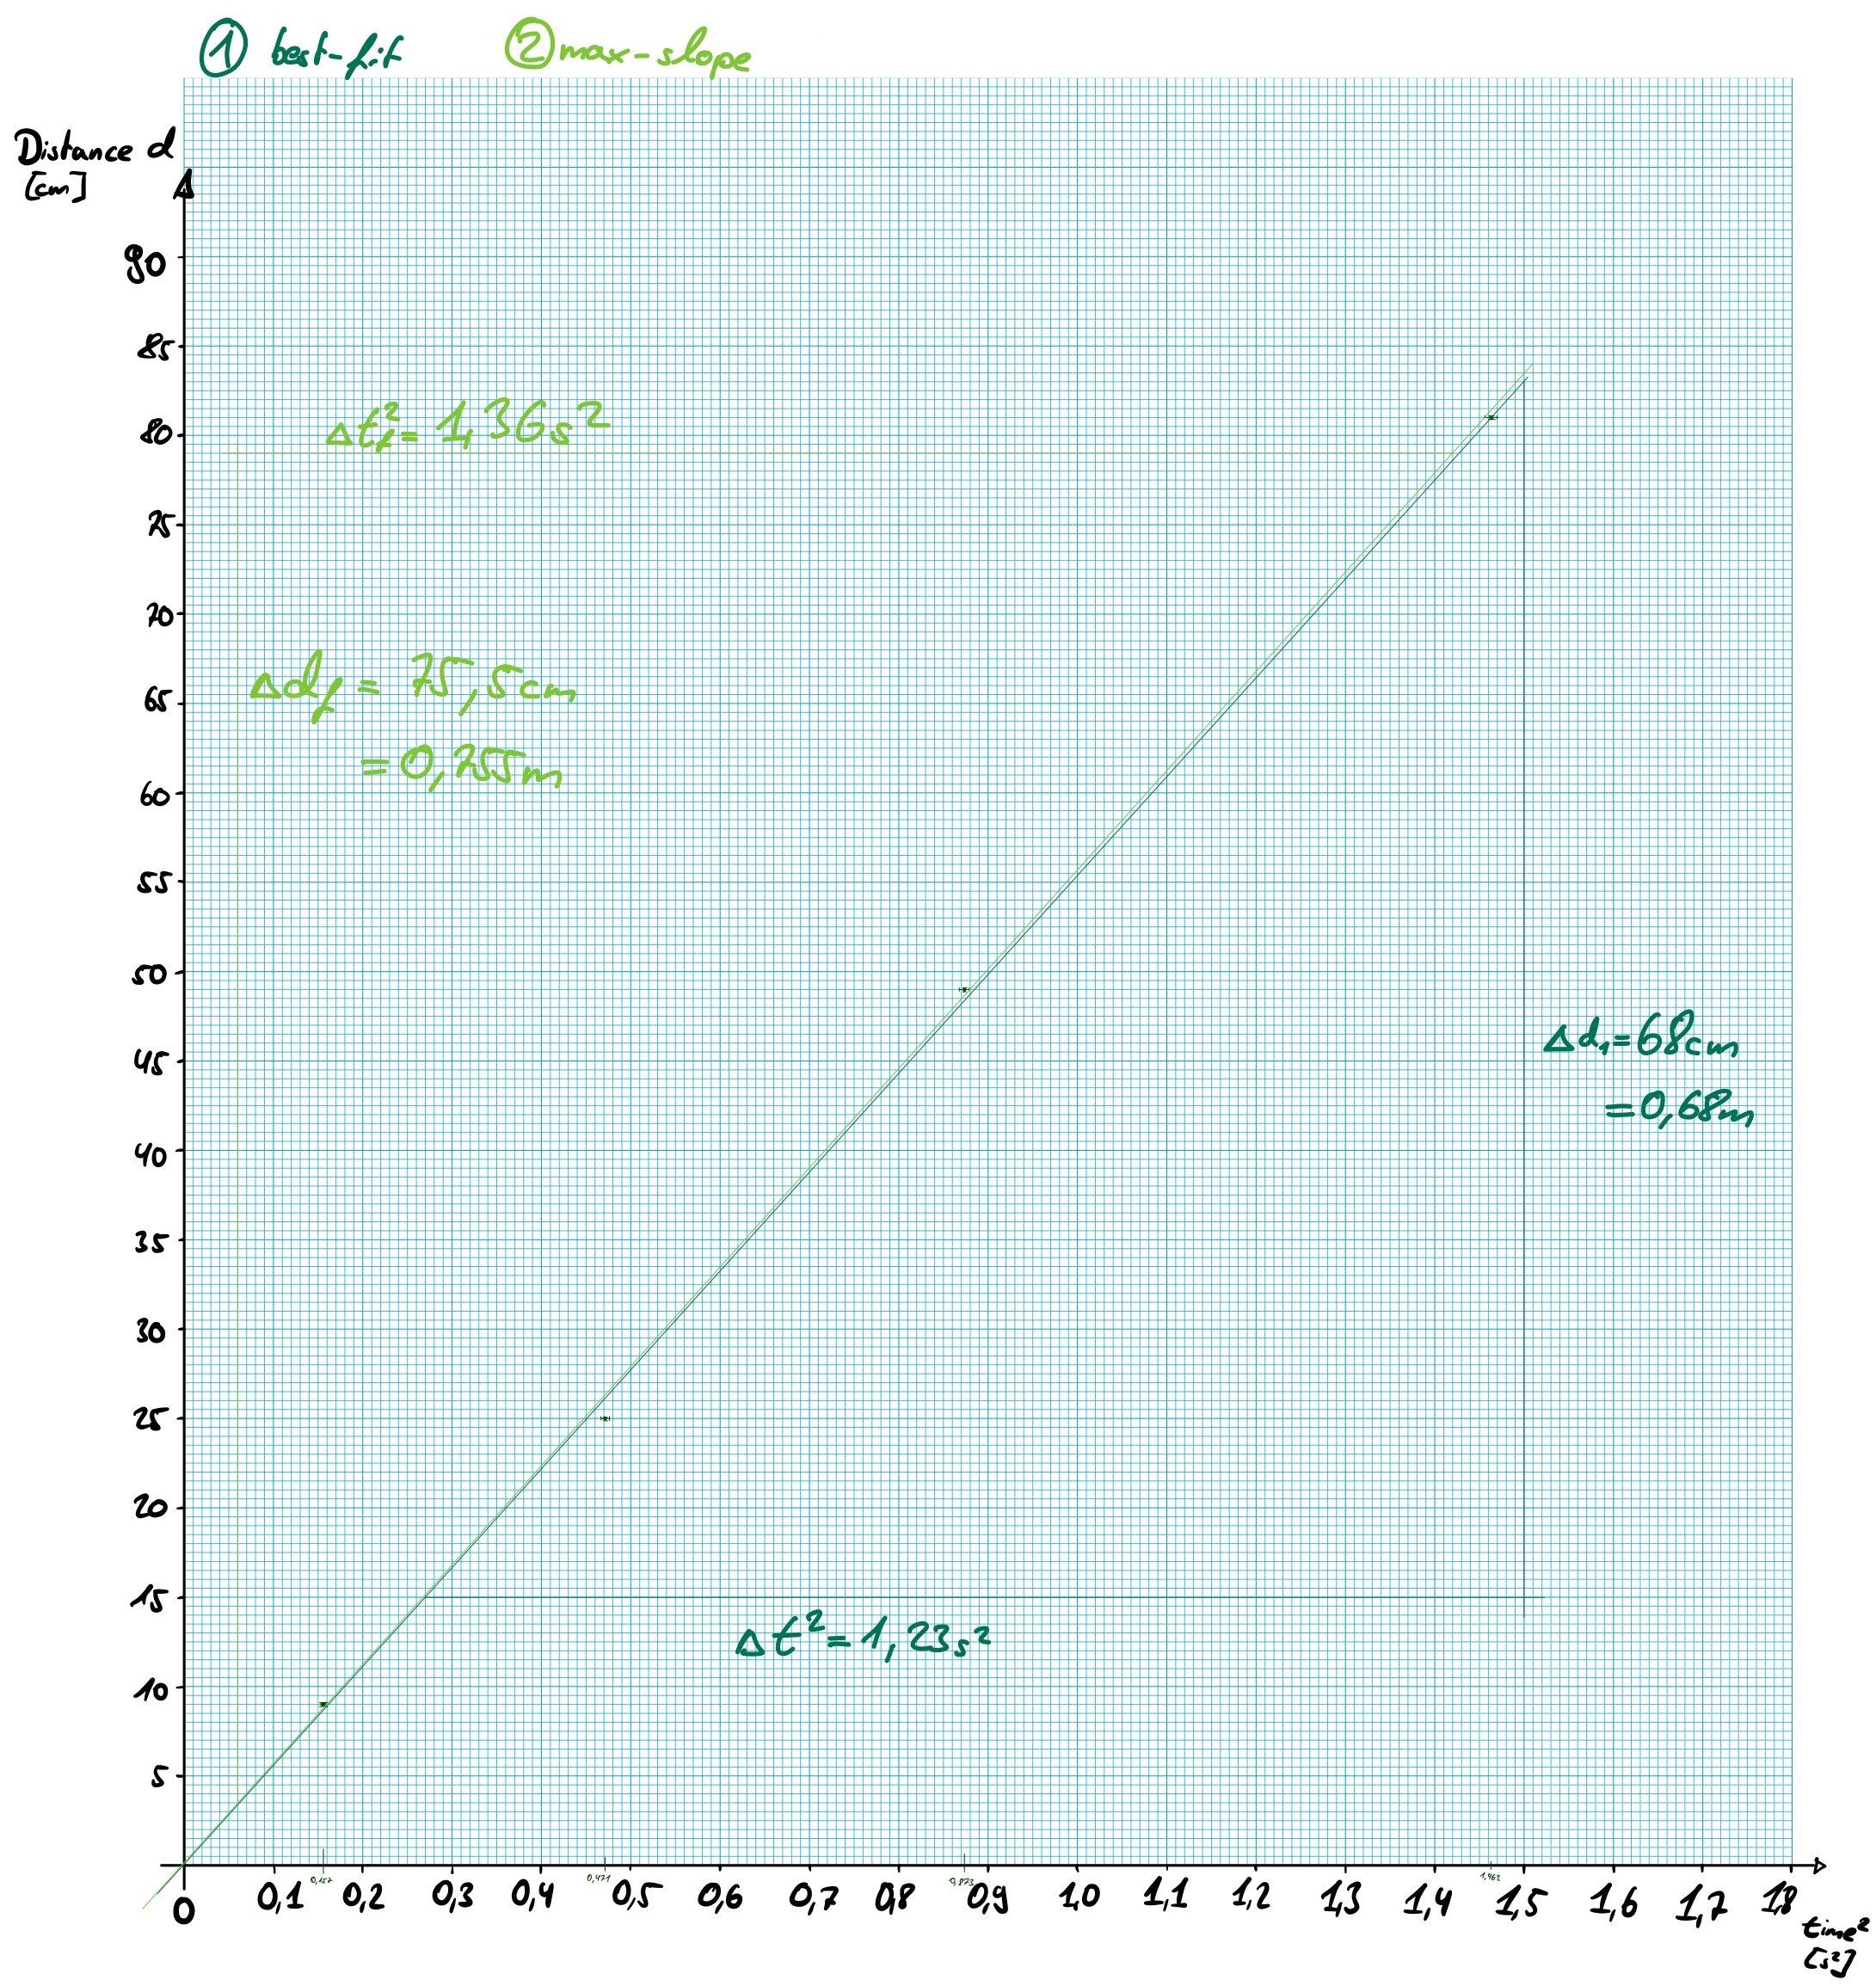
\includegraphics[width=\textwidth]{graphics/dia1.pdf}
    \caption{Abbildungen eines Objekts bei den gegeben Gegenstandsweiten}
\end{figure}

\begin{figure} [p]
    \centering
    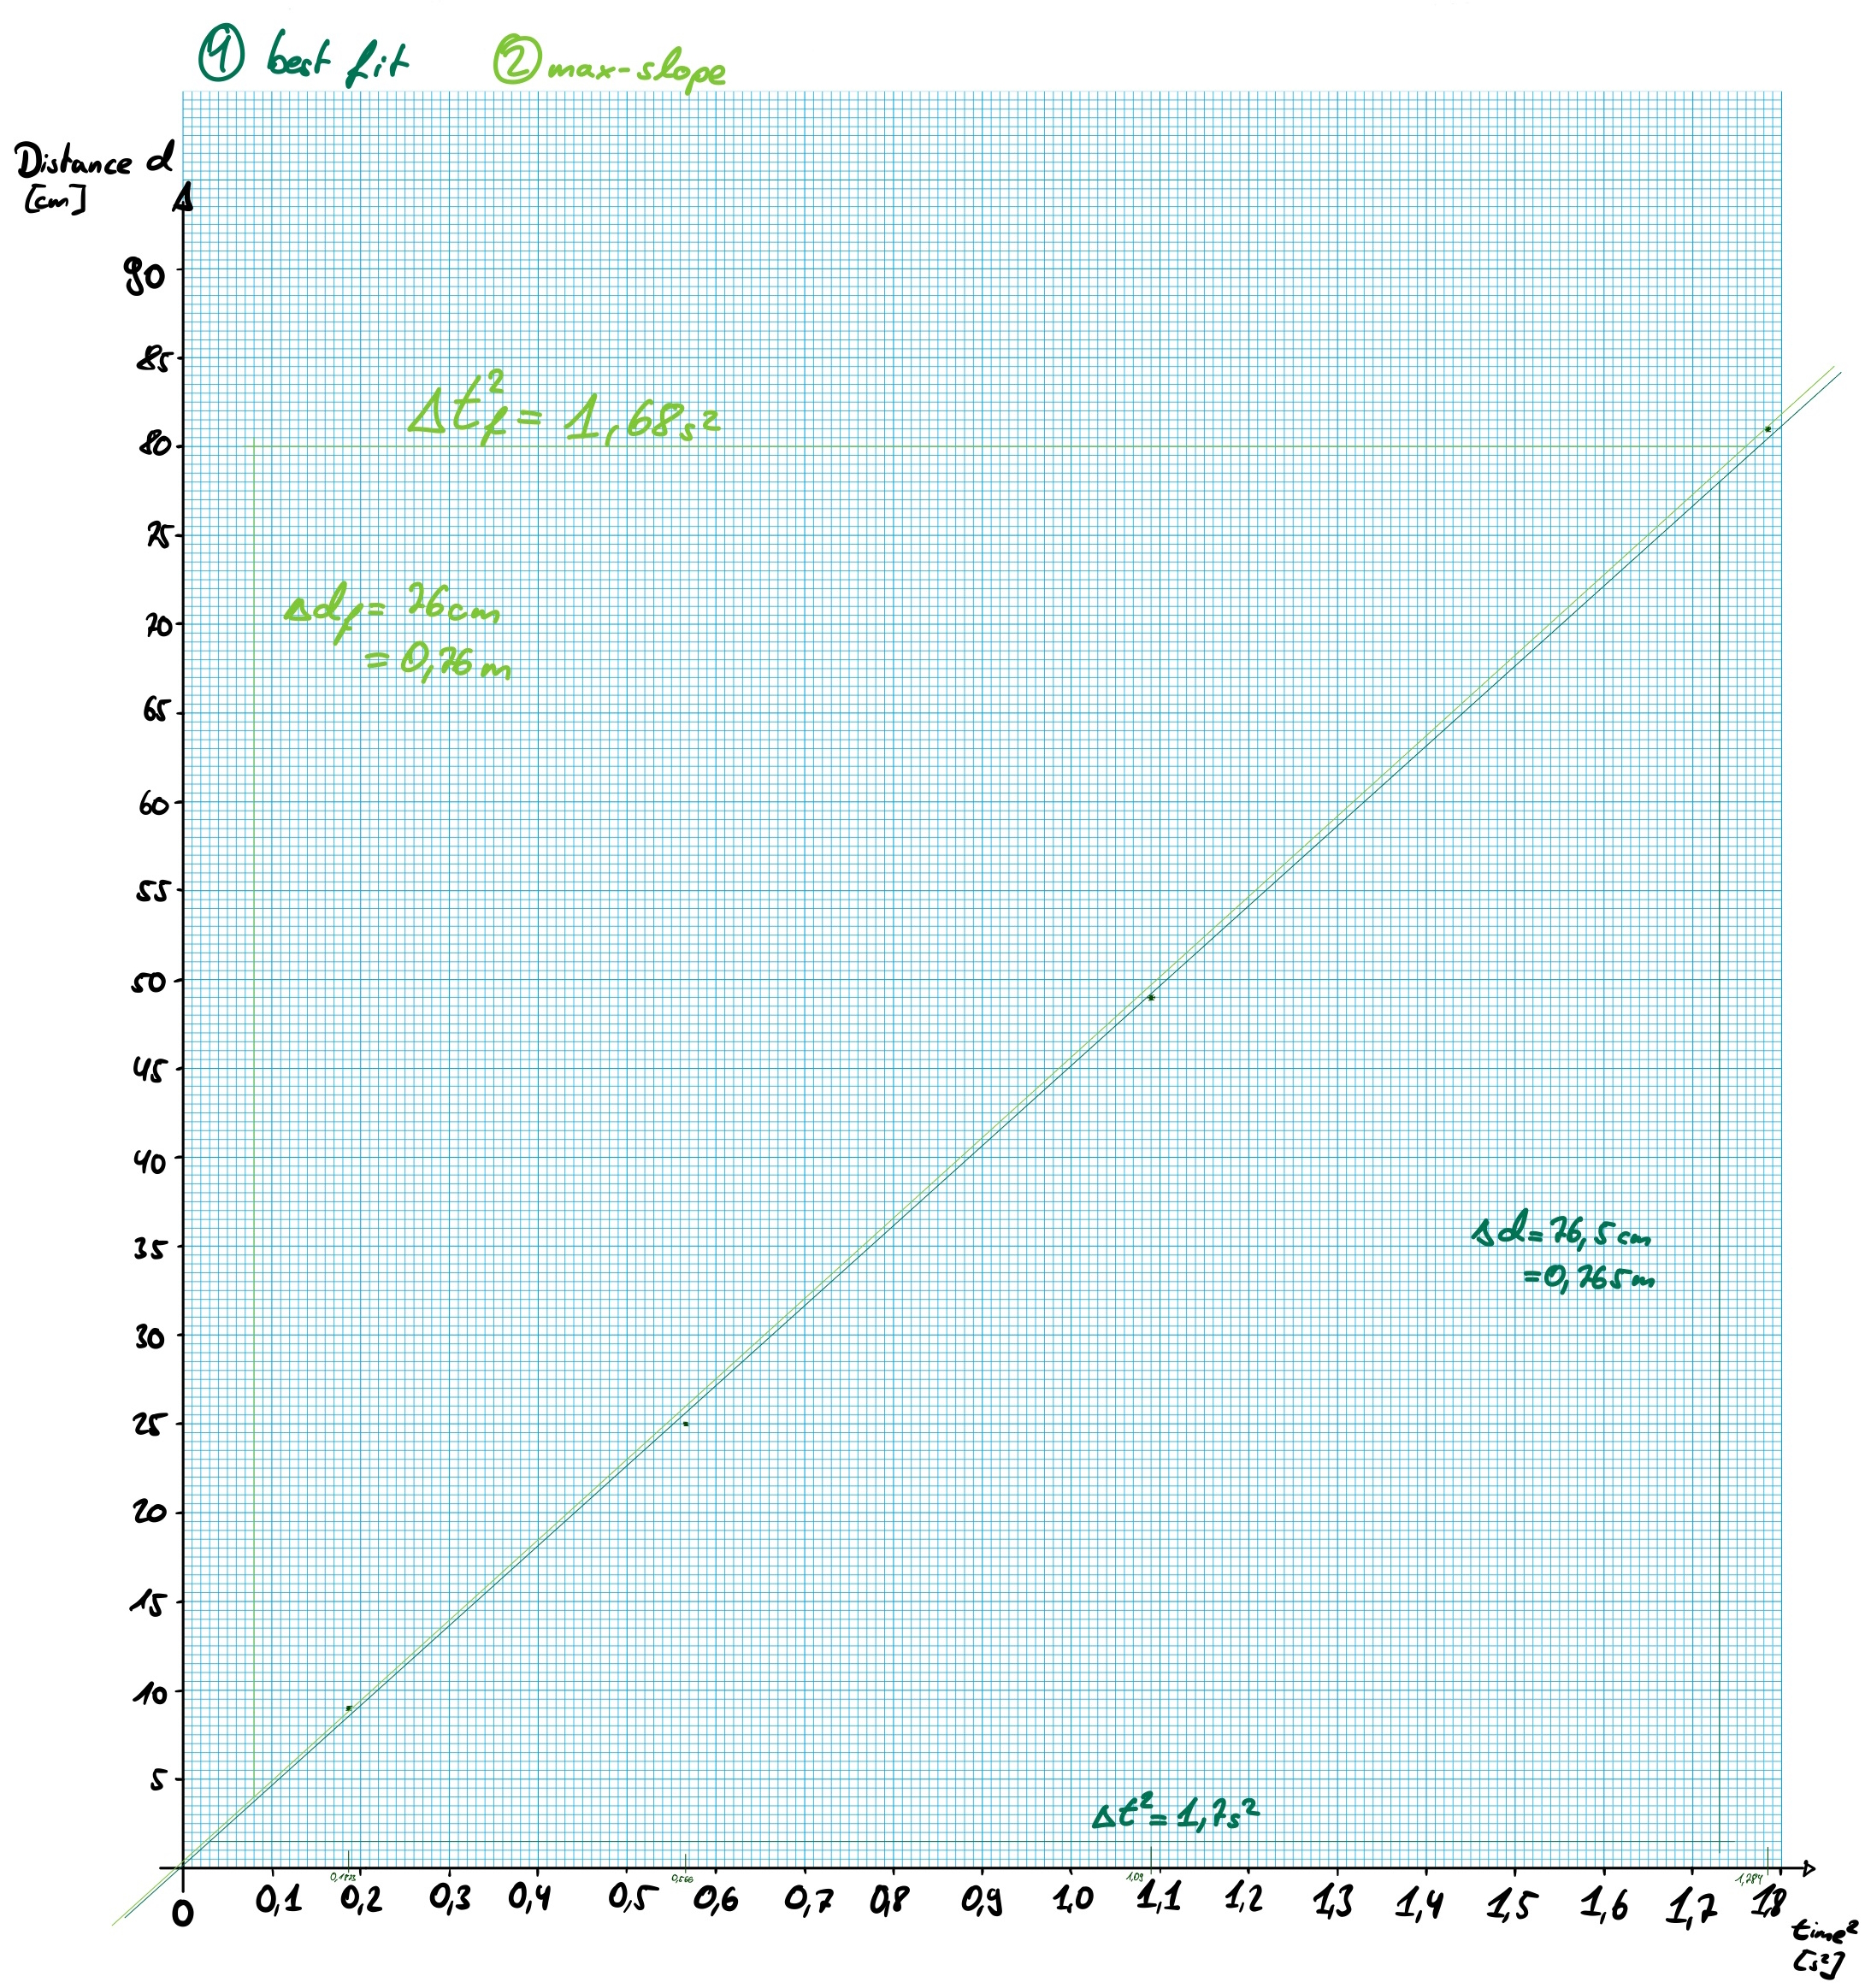
\includegraphics[width=\textwidth]{graphics/dia2.pdf}
    \caption{Diagramm der Bild- und Gegenstandsweiten zur Bestimmung der Brennweite}
\end{figure}

\newpage

\subsection{Zu Aufgabe 2}

Hier geht es nun darum die Brennweite mithilfe des Besselverfahrens zu bestimmen.

Dazu wird zunächst aus den in Tabelle 2 bestimmten Distanzen der Mittelwert $\overline{d}$ sowie dessen Fehler $\Delta \overline{d}$ aus der quadratische Addition des Messfehlers $\Delta d$ und des Standartfehlers des Mittelwerts $\Delta \overline{d}_{\sigma}$ bestimmt. Man erhält:

\begin{equation}
    \begin{split}
        \overline{d} &= 26,23cm \\
        \Delta \overline{d} &= \sqrt{(\Delta d)^2 + (\Delta \overline{d}_{\sigma})^2} = 0,10cm 
    \end{split}
\end{equation}

Nun wendet man Gleichung (3) an und bestimmt den Fehler mit dem Fehlerfortpflanzungsgesetz:

\begin{equation}
    \begin{split}
        f &= \frac{L^2 - {\overline{d}}^2}{4 L} = 12,13cm \\
        \Delta f &= \sqrt{\left( \left( \frac{1}{4} + \frac{\overline{d}^2}{4 L^2} \right) \Delta L \right)^2 + \left( \frac{\overline{d}}{2L} \Delta \overline{d} \right)^2} = 0,04cm \\ \\
        \implies \bm{f} &= \bm{(12,13 \pm 0,04)cm}
    \end{split}
\end{equation}

\subsection{Zu Aufgabe 3}

Analog zur Auswertung von Aufgabe 2 werden die Brennweiten der Linse bei den farbigen Lichtstrahlen bestimmt, um die chromatische Aberration zu untersuchen. Die Werte aus Tabelle 3 für rotes Licht und Tabelle 4 für blaues Licht ergeben:

\begin{equation}
    \begin{split}
        \overline{d}_{rot} &= 25,87cm \\
        \Delta \overline{d}_{rot} &= 0,08cm \\
        \overline{d}_{blau} &= 26,47cm \\
        \Delta \overline{d}_{blau} &= 0,14cm
    \end{split}
\end{equation}

Die Werte für die Brennweiten und deren Fehler sind auch genauso zu berechnen:

\begin{equation}
    \begin{split}
        f_{rot} &= 12,21cm \\
        \Delta f_{rot} &= 0,03cm \\
        f_{blau} &= 12,08cm \\
        \Delta f_{blau} &= 0,04cm \\ \\
        \implies \bm{f_{rot}} &= \bm{(12.21 \pm 0,03)cm} \\
        \bm{f_{blau}} &= \bm{(12,08 \pm 0,04)cm}
    \end{split}
\end{equation}

\subsection{Zu Aufgabe 4}

Der letzte Versuch beinhaltete den Aufbau eines Mikroskops. Im Messprotokoll wurden bereits die folgenden Werte bestimmt:

\begin{equation}
    \begin{split}
        \beta &= 5,25 \pm 0,01 \\
        l_{Bild} &= (0,52 \pm 0,05) mm \\
        l_{Gitter} &= (0,099 \pm 0,010) mm \\
        x &= (3,30 \pm 0,05) cm
    \end{split}
\end{equation}

Dabei sind $\beta$ der Abbildungsmaßstab, $l_{Bild}$ die Größe eines Kästchens im Zwischenbild, $l_{Gitter}$ die Größe eines Kästchens im ursprünglichen Gitter und $x$ der Abstand vom Spalt zum Objekt. Man identifiziert $l_{Gitter}$ als die Gitterkonstante.

Zunächst wird aus den in Tabelle 5 gemessenen Werten für die Spaltbreite der Mittelwert mitsamt Fehler bestimmt:

\begin{equation}
    \begin{split}
        \overline{d} &= 0,23 mm \\
        \Delta \overline{d} &= 0,05mm
    \end{split}
\end{equation}



%Eine erste Berechnung des Auflösungsvermögen geht aus Gleichung (7) hervor. Man verwende $D = \overline{d}$, $g = f = 4cm$ (Brennweite des Objektivs) und $\lambda = 550nm$ (Angabe aus dem Skript):

%\begin{equation}
    %\begin{split}
        %G_{min_1} &= 1,22 \frac{\lambda g}{D} = 0,117mm \\
        %\Delta G_{min_1} &= \sqrt{\left( 1,22 \frac{\lambda g}{D^2} \cdot \Delta D\right)^2} = 0,025mm
    %\end{split} 
%\end{equation}

%\left( \frac{\Delta g}{g} \right)^2 + 
 %0,0021mm

%Setzt man Gleichungen (7) und (8) gleich, lässt sich zunächst der Winkel $\alpha$ bestimmen:

%\begin{equation}
%\begin{split}
    %1,22 \frac{\lambda f}{D} &= 1,22 \frac{\lambda}{2n \sin{\alpha}} \\
    %\implies \alpha &= \arcsin{\left( \frac{D}{2f} \right)} = 0,1647^{\circ}
%\end{split}
%\end{equation}

%Hierbei wird der Brechungsindex für Luft auf $n=1$ gesetzt und für $D$ der Wert der Spaltbreite eingesetzt.

%Der Fehler wird über die Fehlerfortpflanzung berechnet:

%\begin{equation}
%\begin{split}
    %\Delta \alpha &= \sqrt{\left( \frac{\partial}{\partial D} \left( \arcsin{\frac{D}{2f}} \right) \cdot %\Delta D \right)^2} \\
    %&= \frac{1}{2f} \frac{1}{\sqrt{1 - \left( \frac{1}{2f} \right)^2 D^2}} \cdot \Delta D \\
    %&= 0,0006^{\circ}
%\end{split}
%\end{equation}
 
Eine Berechnung des Auflösungsvermögens $G_{min}$ funktioniert mit Gleichung (8), indem man den Winkel $\alpha$ mit Gleichung (9) bestimmt. Man verwende $D = \overline{d}$, $f = 4cm$ (Brennweite des Objektivs), $\lambda = 550nm$ (Angabe aus dem Skript) und $n=1$ in Luft. Als Fehler für die Brennweite $f$ wurde unser Ablesefehler abgeschätzt, ergo $\Delta f = 0,05cm$:

\begin{equation}
    \begin{split}
        \alpha &= \frac{D/2}{f} = 0,0029 \text{rad} \\
        \Delta \alpha &=  \sqrt{\left( \frac{1}{2f} \cdot \Delta D \right)^2 + \left( \frac{D}{2f^2} \cdot \Delta f \right)^2} = 0,0006 \text{rad} \\
        G_{min} &= 1,22 \frac{\lambda}{2n \sin{\alpha}} = 0,116mm \\
        \Delta G_{min} &= \sqrt{\left( 1,22 \lambda \frac{\cos{\alpha}}{\cos{2 \alpha} - 1} \cdot \Delta \alpha \right)^2} = 0,024mm \\ \\
        \implies \bm{G_{min}} &= \bm{(0,116 \pm 0,024)mm}
    \end{split}
\end{equation}

%Wie man sehen kann unterscheiden sich die Werte $G_{min_1}$ und $G_{min_2}$ nur in der letzten angegeben Stelle, was auf Rundungsfehler schließen lässt.

Schlussendlich vergleicht man noch die berechneten Werte für die Gitterkonstante $l_{Gitter}$ und das Auflösungsvermögen $G_{min}$ über den Quotient:

\begin{equation}
    \begin{split}
        \frac{l_{Gitter}}{G_{min}} &= 0,85 \\
        \Delta \frac{l_{Gitter}}{G_{min}} &= \frac{l_{Gitter}}{G_{min}} \sqrt{\left( \frac{\Delta l_{Gitter}}{l_{Gitter}} \right)^2 + \left( \frac{\Delta G_{min}}{G_{min}} \right)^2} = 0,20
    \end{split}
\end{equation}

%Der berechnete Wert ist kleiner als 1 was bedeutet, dass das Gitter mit dem oben stehenden Wert der Spaltbreite $\overline{d}$ nicht mehr abgebildet werden kann. Das passt zur Premisse der Messung, da die Spaltbreite an dem Punkt gemessen wurde, an dem die senkrechten Strukturen des Gitters im Bild gerade so verschwinden.

%---------------PRÄSENTATION DER ENDERGEBNISSE---------------
\newpage

\section{Präsentation der Endergebnisse}

Zusammenfassend wurden bei diesem Versuch folgende Ergebnisse erziehlt:

Zunächst wurde mithilfe von Gegenstands- und Bildweitemessungen die Brennweite einer Achromatlinse bestimmt:

\begin{equation}
    \bm{f_{graph} = (10,1 \pm 0,4)cm}
\end{equation}

Anschließend wurde mit dem Besselverfahren die Brennweite einer bikonvexen Linse bestimmt:

\begin{equation}
    \bm{f} = \bm{(12,13 \pm 0,04)cm}
\end{equation}

Mit demselben Verfahren wurden dann die Brennweiten der gleichen bikonvexen Linse einmal bei blauem und einmal bei rotem Licht untersucht:

\begin{equation}
    \begin{split}
        \bm{f_{rot}} &= \bm{(12.21 \pm 0,03)cm} \\
        \bm{f_{blau}} &= \bm{(12,08 \pm 0,04)cm}
    \end{split}
\end{equation}

Zuletzt wurde bei einem Aufbau eines Mikroskops das Auflösungsvermögen bestimmt und mit der Gitterkonstante verglichen:

\begin{equation}
\begin{split}
    \bm{G_{min}} &= \bm{(0,116 \pm 0,024)mm} \\
    \bm{\frac{l_{Gitter}}{G_{min}}} &= \bm{0,85 \pm 0,20}
\end{split}
\end{equation}

%---------------ZUSAMMENFASSUNG UND DISKUSSION---------------
\newpage

\section{Zusammenfassung und Diskussion}

In diesem Versuch wurden auf zwei verschiedenen Wegen Brennweiten von Linsen bestimmt, diese quantitativ auf die chromatische sowie qualitativ auf die shphärische Aberration untersucht und das Auflösungsvermögen eines Mikroskops bestimmt. 

Dabei lieferten die Berechnungen und Beobachtungen fast immer erwartete Ergebnisse. Bei den ersten drei Teilen ergaben die Werte im Vergleich miteinander immerzu Sinn und passten mit unserem physikalischen Verständnis überein. 

Bei Teil Eins lässt sich das mit der berechneten Sigmaabweichung von $\sigma = 0,63$ zwischen dem grafisch und rechnerisch bestimmten Wert für $f$ begründen, die sogar noch unterhalb der $1\sigma$-Grenze liegt. 

Beim zweiten Teil gab es zwar keine Angaben zum Vergleich, der berechnete Wert von $f = (12,13 \pm 0,04)cm$ erscheint im Kontext des Versuchs aber als sinnvoll und passt zu den Ergebnissen von Teil drei, bei dem wie erwartet die Brennweite für rotes Licht länger als die für blaues Licht berechnet wurde und der Wert ohne Farbfilter zwischen den beiden liegt. Physikalisch lässt sich diese Beobachtung damit begründen, dass blaues Licht eine kürzere Wellenlänge hat und somit stärker gebrochen wird. Bei rotem Licht ist dann genau das Gegenteil der Fall. \\
Die Beobachtung der sphärischen Aberration erfolgte hier dann nur qualitiativ, ergab aber, dass der Abstand $d$ im Schnitt bei der Ringblende größer und bei der Lochblende kleiner wird. Das sorgt im Endeffekt für eine kleinere Brennweite bei der Lochblende im Vergleich zur Ringblende was bestätigt, dass achsenferne Lichtbündel tatsächlich stärker gebrochen werden als achsennahe. 

Nur bei Aufgabenteil Vier ergab sich ein nicht vorhergesehenes Ergebnis. Hier wurde die Gitterkonstante als $l_{Gitter} = (0,099 \pm 0,010) mm$ und das Auflösungsvermögen als $G_{min} = (0,116 \pm 0,024)mm$ bestimmt, was zum Quotienten $\frac{l_{Gitter}}{G_{min}} = 0,85$ führte, der eigentlich größer als 1 sein sollte. Fehlerquellen könnten hier eine falsche Messung des Strichabstands beim Zwischenbild, eine ungenaue Einstellung der Bildweite von 25cm oder ein Messfehler bei Bestimmung der Spaltbreite sein. Auch ist die etwas sperrige Bedienung des Schiebers zur Einstellung der Spaltbreite hier erwähnenswert, dieser blieb nämlich gerne mal etwas hängen und motivierte somit eventuell zu psychologischen Fehlern und Fehleinschätzungen. Zudem war insgesamt die Abschätzung, ab wann die senkrechten Strukturen des Gitters nicht mehr zu erkennen waren, recht schwierig. Dennoch lässt sich erwähenen, dass es theoretisch Werte größer als 1 gibt, die, vorausgesetzt sie haben einen ähnlichen Fehler wie der bestimmte Wert $\Delta \frac{l_{Gitter}}{G_{min}}$, noch innerhalb der $1\sigma$-Umgebung von unserem Quotienten liegen. Die Abweichung ist also theoretisch hier nicht signifikant, aber das Ergebnis, dass $l_{Gitter}$ kleiner ist als $G_{min}$, bleibt nicht richtig. 

Während des Versuchs wurden noch nach dem gleichen Verfahren wie im vierten Teil die Spaltbreiten bei rotem und blauen Licht qualitativ betrachtet. Man konnte feststellen, dass die Spaltbreite beim blauen Licht etwas kleiner und beim roten Licht etwas größer wird. 

Allgemein lassen sich trotz der weitgehend vereinbaren Ergebnisse noch folgende Kritikpunkte und potenzielle Fehlerquellen nennen.

Zunächst sind allgemeine Messfehler, Ablesefehler und Gerätefehler zu nennen. Während Messfehler bei uns nicht aufgefallen sind und wir Ablesefehler im allgemeinen gut abschätzen konnten, gab es bei diesem Versuch keine Angaben über Gerätefehler der bereitgestellten Materialien, wie z.B. der Brennweite der Linse, wo nur der von uns abgeschätzte Ablesefehler der Skala verwendet werden konnte. 

Eine weitere nennenswerte potentielle Fehlerquelle war der Schirm, auf dem in den ersten drei Versuchsteilen das Bild betrachtet wurde. Dieser war nämlich dadurch, dass sich die Plastikbeschichtung auf dem Metall etwas zu lösen begann, an manchen Stellen sichtbar gewölbt. Wie im Messprotokoll erwähnt haben wir hierfür einen etwas größeren Fehler abgeschätzt, dennoch ist unsere Abschätzung sicherlich nicht zwangsweise perfekt.   

Des Weitern lässt sich vermerken, dass die Abschätzung der richtigen Position, bei der das Bild scharf ist, nach persönlichem Ermessen erfolgte und somit nicht perfekt sein kann, da der Unterschied zwischen einem scharfen und einem gerade so nicht mehr scharfen Bild häufig schwer zu differenzieren war. 

Zum Schluss lässt sich das Fazit ziehen, dass trotz den genannten potenziellen Fehlerquellen alle Resultate, bis auf die Thematisierten in Teil Vier, zu Werten ohne signifikante Abweichungen sowie zu Beobachtungen, die nicht im Konflikt mit unseren Erwartungen stehen würden, und somit zu sinnvollen Versuchsergebnissen führten.

\end{document}

